\documentclass{easychair}

% \usepackage{doc}
\usepackage{setspace}
\usepackage{verbatim}

%----Making things more compact
\newcommand{\smalltt}[1]{\small \texttt{#1}}
\newenvironment{packed_itemize}{
\vspace*{-0.2em}
\begin{itemize}
\setlength{\partopsep}{0pt}
\setlength{\itemsep}{1pt}
\setlength{\parskip}{0pt}
\setlength{\parsep}{0pt}
}{\end{itemize}}
\newenvironment{packed_enumerate}{
\vspace*{-0.2em}
\begin{enumerate}
\setlength{\partopsep}{0pt}
\setlength{\itemsep}{1pt}
\setlength{\parskip}{0pt}
\setlength{\parsep}{0pt}
}{\end{enumerate}}
% \renewcommand{\textfraction}{0.07}
% \renewcommand{\topfraction}{0.9}
% \renewcommand{\bottomfraction}{0.9}
% \renewcommand{\floatpagefraction}{0.66}
% \setlength{\floatsep}{2.0pt plus 2.0pt minus 2.0pt}
% \setlength{\textfloatsep}{5.0pt plus 2.0pt minus 0.0pt}

\title{Stepping Stones in the TPTP World}

\author{
  Geoff Sutcliffe
}

\institute{
  University of Miami,
  Miami, USA\\
  \email{geoff@cs.miami.edu}\\
}

\authorrunning{Geoff Sutcliffe}
\titlerunning{Stepping Stones in the TPTP World}

\begin{document}
\maketitle

%--------------------------------------------------------------------------------------------------
\begin{abstract}
The first release of the TPTP problem library was made on Friday 12th November 1993. 
Since then the TPTP World (once gently referred to as the ``TPTP Jungle'') has evolved into a 
well established infrastructure that supports research, development, and deployment of ATP systems.
There have been some key developments that helped make the TPTP World a success: 
the first TPTP problem library that was first released in 1993, 
the CADE ATP System Competition (CASC) that was conceived after CADE-12 in Nancy in 1994, 
the problem difficulty ratings that were added in 1997, 
the current TPTP language that was adopted in 2003, 
the SZS ontologies that were specified in 2004, 
the TSTP solution library that was built starting around 2005, 
the Specialist Problem Classes (SPCs) used to classify problems from 2010, 
the SystemOnTPTP service that was offered from 2011, 
and 
the StarExec service that started in 2013. 
This talk reviews these stepping stones in the development of the TPTP World.
\end{abstract}
%--------------------------------------------------------------------------------------------------
\section{Introduction}
\label{Introduction}

The TPTP World \cite{Sut10,Sut17} is a well established infrastructure that supports research, 
development, and deployment of ATP systems.
Salient components of the TPTP World are
the TPTP problem library \cite{Sut09}, 
the TSTP solution library \cite{Sut10}, 
the TPTP languages \cite{SS+06}, 
the SZS ontologies \cite{Sut08-KEAPPA},
the Specialist Problem Classes (SPCs) and problem difficulty ratings \cite{SS01},
and the CADE ATP System Competition (CASC) \cite{Sut16}.
StarExec \cite{SST14} and SystemOnTPTP \cite{Sut00-CADE-17} provide computational support for
the TPTP World.
There are dependencies between these parts of the TPTP World, as shown in 
Figure~\ref{Dependencies}, forming a series of "stepping stones" from key starting points
through to happy users.

\begin{figure}[htbp]
\centering
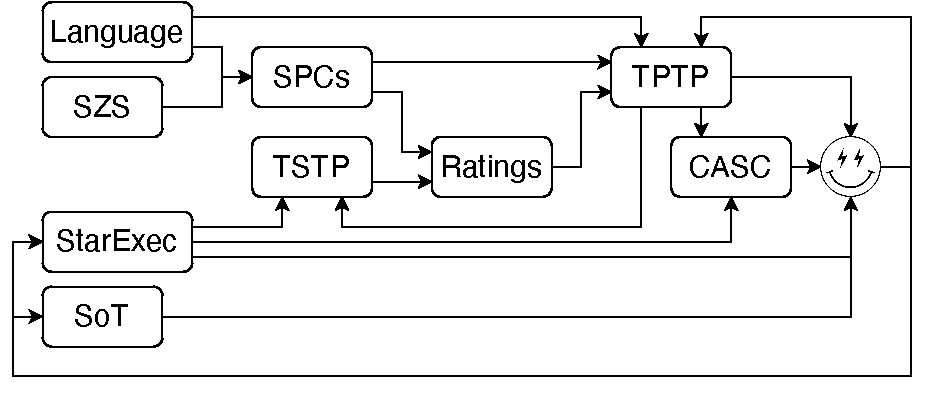
\includegraphics[width=0.75\textwidth]{Dependencies.pdf}
\caption{Dependencies between the Stepping Stones}
\label{Dependencies}
\end{figure}

Various parts of the TPTP World have been deployed in a range of applications,
in both academia and industry.
Since the first release of the TPTP problem library in 1993, many researchers have used the 
TPTP World as an appropriate and convenient basis for ATP system research and development. 
Over the years the TPTP World has provided a platform upon which ATP users have presented their 
needs to ATP system developers, who have then adapted their ATP systems to the users’ needs.
The web page {\smalltt{\url{https://www.tptp.org}}} provides access to all components.

\paragraph{This paper is organized as follows:}

%--------------------------------------------------------------------------------------------------
\section{The TPTP Languages}
\label{TPTP}

The TPTP language \cite{Sut23-IGPL} is one of the keys to the success of the TPTP World.
The language is used for writing both problems and solutions,
which enables convenient communication between systems. 
% It also enables tool exchange, tool integration, and comparable experimental results.
Originally the TPTP World supported only first-order clause normal form (CNF)
\cite{SS98-JAR}.
Over the years full first-order form (FOF)
\cite{Sut09}, 
typed first-order form (TFF)
\cite{SS+12,BP13-TFF1}, 
typed extended first-order form (TXF)
\cite{SK18}, 
typed higher-order form (THF)
\cite{SB10,KSR16}, 
and non-classical forms (NTF)
\footnote{%
There are many ``non-classical logics'', including multi-valued logics \cite{Aug17},
paraconsistent logics \cite{Pri02}, relevance logics \cite{AB75}, etc.
In this work we are interested in those that admit Kripke interpretation \cite{Kri63},
e.g., modal logics \cite{BBW06}.}
\cite{SF+22} 
have been added.
A general principle of the TPTP language is ``we provide the syntax, you provide the semantics''.
As such, there is no a priori commitment to any semantics for the languages, although in almost 
all cases the intended logic and semantics are well known.
All the typed forms include constructs for arithmetic.
TF0 \cite{SS+12}, the monomorphic subform of TFF, is used in this work (see Section~\ref{TF0}).

The top level building blocks of the TPTP language are {\em annotated formulae}.
An annotated formula has the form:\\
\hspace*{0.5cm}{\em language}{\tt (}{\em name}{\tt ,}
{\em role}{\tt ,}
{\em formula}{\tt ,}
{\em source}{\tt ,}
{\em useful\_info}{\tt )}\\
The {\em language}s supported are {\smalltt{cnf}} (clause normal form), {\smalltt{fof}}
(first-order form), {\smalltt{tff}} (typed first-order form), and {\smalltt{thf}}
(typed higher-order form).
The {\em role}, e.g., {\smalltt{axiom}}, {\smalltt{lemma}}, {\smalltt{conjecture}},
defines the use of the formula in an ATP system.
In a {\em formula}, terms and atoms follow Prolog conventions
-- functions and predicates start with a lowercase letter or are {\tt '}single quoted{\tt '}, and 
variables start with an uppercase letter.
The language also supports interpreted symbols, which either start with a {\tt \$}, e.g., 
the truth constants {\smalltt{\$true}} and {\smalltt{\$false}}, or are composed of 
non-alphabetic characters, e.g., integer/rational/real numbers such as 27, 43/92, -99.66.
The logical connectives in the TPTP language are
{\tt !}, {\tt ?}, {\tt {\raisebox{0.4ex}{\texttildelow}}}, {\tt |}, {\tt \&}, {\tt =>}, {\tt <=},
{\tt <=>}, and {\tt <{\raisebox{0.4ex}{\texttildelow}}>},
for the mathematical connectives
$\forall$, $\exists$, $\neg$, $\vee$, $\wedge$, $\Rightarrow$, $\Leftarrow$, $\Leftrightarrow$, 
and $\oplus$ respectively.
Equality and inequality are expressed as the infix operators {\tt =} and {\tt !=}.
The {\em source} and {\em useful\_info} are optional.

%--------------------------------------------------------------------------------------------------
\section{Conclusion}
\label{Conclusion}

This paper 

Currently this work is being extended to 

%--------------------------------------------------------------------------------------------------
\bibliographystyle{plain}
\bibliography{Bibliography.bib}
%--------------------------------------------------------------------------------------------------
\end{document}
%--------------------------------------------------------------------------------------------------
